\documentclass[border=6pt]{standalone}
\usepackage{amsmath}
\usepackage{tikz}
\usetikzlibrary{arrows.meta,decorations.pathmorphing,calc}
\begin{document}
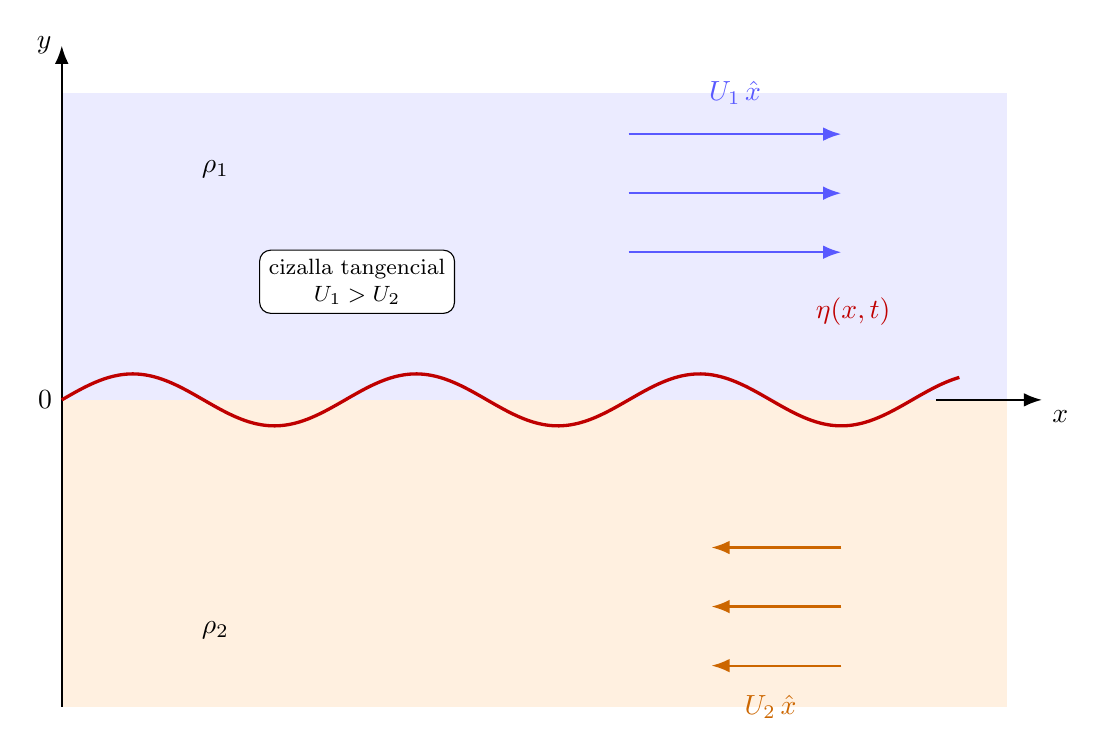
\begin{tikzpicture}[>=Latex,scale=1.5]

% regiones separadas por la interfaz ondulada (relleno simple rect, la onda va encima)
\fill[blue!8]   (0,0) rectangle (8,2.6);
\fill[orange!12] (0,-2.6) rectangle (8,0);

% eje y (izquierda)
\draw[->,thick] (0,-2.6) -- (0,3.0) node[left] {$y$};
\node[left] at (0,0) {$0$};

% interfaz perturbada eta(x,t): onda senoidal roja gruesa sobre la frontera y=0
\draw[very thick,red!75!black,smooth,samples=140,domain=0:7.6]
      plot (\x,{0.22*sin(\x*150)});
% flecha-eje x al final de la interfaz
\draw[->,thick] (7.4,0) -- (8.3,0) node[below right] {$x$};
\node[red!75!black] at (6.7,0.75) {$\eta(x,t)$};

% region superior: rho1, U1 (rapido, derecha)
\node at (1.3,1.95) {$\rho_1$};
\foreach \yy in {1.25,1.75,2.25}{\draw[->,blue!65,thick] (4.8,\yy) -- (6.6,\yy);}
\node[blue!65] at (5.7,2.6) {$U_1\,\hat{x}$};

% region inferior: rho2, U2 (lento/opuesto)
\node at (1.3,-1.95) {$\rho_2$};
\foreach \yy in {-1.25,-1.75,-2.25}{\draw[->,orange!80!black,thick] (6.6,\yy) -- (5.5,\yy);}
\node[orange!80!black] at (6.0,-2.6) {$U_2\,\hat{x}$};

% nota condicion de cizalla
\node[draw,rounded corners,fill=white,font=\footnotesize,align=center] at (2.5,1.0)
  {cizalla tangencial\\ $U_1 > U_2$};

\end{tikzpicture}
\end{document}
